% !TEX encoding = UTF-8 Unicode

\linespread{1.7}
\chapter{Calibration of the Near-surface Seismic Structure in the SCEC Community Velocity Model Version 4}
\linespread{2.0}
%\newrefsection
\label{chap:vs30}

\graphicspath{{/Users/zhh076/work/PhD_way/vs30/}}

The near-surface seismic structure (to a depth of about 1000 m), particularly the shear-wave velocity ($V_S$), can strongly affect the propagation of seismic waves, and therefore must be accurately calibrated for ground motion simulations and seismic hazard assessment. The $V_S$ of the top ($< 300$ m) crust is often well-characterized from borehole studies, geotechnical measurements, and water and oil wells, while the velocities of the material deeper than about 1000 m are typically determined by tomography studies. However, in regions lacking information on shallow lithological stratification, typically rock sites outside the sedimentary basins, the material parameters between these two regions are typically poorly characterized due to resolution limits of seismic tomography. When the alluded geological constraints are not available, models, such as the Southern California Earthquake Center Community Velocity Models (CVMs), default to regional tomographic estimates that do not resolve the uppermost $V_S$ values, and therefore deliver unrealistically high shallow $V_S$ estimates. A widely-used method for incorporating the near-surface earth structure is implemented in CVMs by applying a generic overlay based on measurements of time-averaged $V_S$ in top 30 m ($V_{S30}$) to taper the upper part of the model to merge with tomography at certain depth (e.g., 350 m). However, our 3D simulations of the 2014 $M_w$ 5.1 La Habra earthquake in the Los Angeles area using the CVM-S4.26.M01 model significantly underpredict low-frequency (< 1 Hz) ground motions at sites subject to the generic overlay (``taper''). On the other hand, extending the $V_{S30}$-based taper of the shallow velocities down to a depth of about 1000 meters improves the fit between our synthetics and seismic data at those sites, without compromising the fit at well constrained sites. We explore various tapering depths, demonstrating increasing amplification as the tapering depth increases, and the model with 1000 m tapering depth yields overall favorable results. Effects of varying anelastic attenuation are small compared to effects of velocity tapering. Although a uniform tapering depth is adopted in the models, we observe some spatial variabilities that may further improve our method.


%%%%%%%%%%%%%%%%%%%%%%%%%%
\section{Introduction} \label{vs30:intro}
Ground motion amplification due to the near-surface structure is widely accepted and well-studied \citeg{gilbertSanFranciscoEarthquake1907,fieldModifiedGroundMotionAttenuation2000}, and needs to be incorporated in numerical  simulations of earthquakes to produce accurate ground motion results. Theoretical analyses have shown that the near-surface shear-wave velocity ($V_S$) can exert strong control on spectral amplification \citep{joynerEffectQuaternaryAlluvium1981,booreEstimationGroundMotion1991,andersonControlStrongMotion1996,dayRMSResponseOnedimensional1996}. The time-averaged shear-wave velocity in the upper 30 m ($V_{S30}$) is routinely used as a representation of the site condition in ground motion prediction models and building codes \citep{borcherdtEstimatesSiteDependentResponse1994,bozorgniaNGAWest2ResearchProject2014,internationalcodecouncil2015IBCInternational2014}. Several methods have been proposed for estimating $V_{S30}$ from topography \citep{waldTopographicSlopeProxy2007}, supplemented with near-surface geological information \citep{thompsonVS30MapCalifornia2014,willsNextGeneration302015}. However, despite the continuing advancement in the $V_{S30}$-based methodologies by the seismic hazard community \citeg{thompsonVS30MapCalifornia2014,heathGlobalHybrid302020},  estimating $V_{S30}$ at high resolution remains a difficult task and it is noted that $V_{S30}$ is not a good single proxy for the estimation of site amplification \citeg{steidlSiteResponseSouthern2000,leeShouldAverageShearwave2010,shingakiEvaluationPerformanceSite2018}. Other empirical methodologies provide additional predictive capability for shallow low-velocity amplification, normally constrained by sediment depth, which is parameterized using the depth to the 1 km/s ($z_1$) or 2.5 km/s ($z_{2.5}$) $V_S$ horizon \citeg{abrahamsonSummaryASK14Ground2014,booreNGAWest2EquationsPredicting2014,campbellNGAWest2GroundMotion2014}. Nonetheless, these empirical methods, oftentimes dependent on $V_{S30}$, have similar limitations with $V_{S30}$ that depth-dependent and lateral velocity variations are insufficiently accounted for.

While the current approximations to correct for site effects represent great progress in ground motion estimation, a fully physics-based approach to computing ground motion offers opportunities for further improvements. The physics-based approach entails difficult challenges as well, and remains a long-term goal. In such an approach, the full wavefield is computed deterministically, to maximum frequencies that are sometimes up to 5 Hz or higher, using a 3D velocity model that includes observationally constrained heterogeneities \citep{savranGroundMotionSimulation2019,withersGroundMotionIntraevent2019,hu05HzDeterministic2021}. A necessary ingredient in producing accurate synthetic seismograms using physics-based simulations is an accurate velocity model for the model region. Community Velocity Models (CVMs) have been developed for such purpose, e.g., the Southern California Earthquake Center (SCEC) CVMs \citep{smallSCECUnifiedCommunity2017}, the Cascadia CVM \citep{stephensonCascadiaSubductionZone2017} and the Subsurface Structure Model maintained by the Japan Seismic Hazard Information Station \citep{fujiwaraJSHISINTEGRATEDSYSTEM2017}. These velocity models are often generated by combining 3D tomographic inversion from seismic waves \citep{tapeAdjointTomographySouthern2009,tapeSeismicTomographySouthern2010,leeFull3DTomographyCrustal2014} with shallow geotechnical information (e.g., $V_{S30}$). The spatial resolution of large-scale tomographic studies is generally limited by the density of ray paths, distribution of high-quality measurements, or intrinsic nonuniqueness of inversion, particularly in the upper \textasciitilde 1000 m of the crust. For example, \citet{linThreedimensionalCrustalSeismic2007} had a vertical grid spacing of 3 km and only resolved $> 1$ km velocity contrasts in their tomographic inversion using P and S wave arrival time, the full-3D seismic waveform tomography conducted by \citet{leeFull3DTomographyCrustal2014} can reach at best 1 km resolution in the center of the inverted region, and \citet{qiuEikonalTomographySouthern2019} found the top 3 km is poorly constrained in their Eikonal tomography using ambient noise cross correlations.


Shallow velocity structure, e.g. S-wave impedance and scattering, has an significant role in modifying ground motion amplification and duration \citeg{graves1995preliminary,andersonControlStrongMotion1996,imperatoriBroadbandNearfieldGround2013}. Specifically, 1D theoretical analysis by \citet{dayRMSResponseOnedimensional1996} suggests that the smoothed amplification spectrum is principally determined by shallow $V_S$, above roughly the depth of half the smoothing bandwidth expressed as a wavelength. Over a \textasciitilde 0.5 Hz bandwidth and typical Southern California rock site $V_S$ values, the analysis predicts that the $V_S$ structure above about 1000 m will have a disproportionately strong effect on ground motion. Therefore, resolving the shallow velocity structure is essential in accurate predictions of ground motions. In SCEC CVMs, velocities and densities in the top 300 m within the basins are constrained by geotechnical and geophysical data, such as seismic reflection surveys, borehole seismic records and gravity data, and in the deeper basins are estimated either from empirical age- and depth-consolidation rules based on water and oil wells and geological studies, or sonic logs and reflection/refraction profiles from the oil industry \citep{magistraleGeologybased3DVelocity1996,magistraleSCECSouthernCalifornia2000,sussWaveSeismicVelocity2003}. Unfortunately, outside and below the basins (typically rock sites), CVMs simply assign interpolated results from regional tomography studies. Additional data constraints on shallow velocity structure, including seismic refraction studies \citeg{teagueMeasuredVsPredicted2018} or borehole logs \citeg{stellerNewBoreholeGeophysical1996,thompsonTaxonomySiteResponse2012} are rare in these regions.

Where location-specific constraints are lacking, previous studies have attempted to use generic models to bridge the gap between data constraints at shallow (< \textasciitilde 30 m) and deeper (> \textasciitilde 1000 m) depths. For example, \citet{booreSiteAmplificationsGeneric1997} generated a continuous depth-dependent $V_S$ function based on 3 different intervals. The $V_S$ profile in the upper 30 m was constructed from interpolated shallow average arrival times. At depths below 4 km, $V_S$ was estimated from the P-wave velocity ($V_P$), measured from earthquake location studies and velocity surveys, on the assumption of a fixed Poisson ratio at 0.25. Finally, the shallow and deeper $V_S$ were connected using two power-law functions. \citet{elyVs30derivedNearsurfaceSeismic2010} proposed a generalized method that derives the surface $V_S$ by linearly scaling $V_{S30}$ and then interpolates velocities with depths until converging to the original tomography model at a certain depth, a scheme which has been implemented in some of the SCEC CVMs. We will use the term ``tapering'' to denote the replacement of (poorly constrained) site-specific CVM values by a generic function of depth that merges smoothly with the original CVM at some depth $z_T$. \citet{elyVs30derivedNearsurfaceSeismic2010} proposed a value of 350 m for $z_T$, based on qualitative comparison between synthetic and seismic records from the 2008 $M_w$ 5.4 Chino Hills, CA, earthquake.

In this study, we quantify the accuracy of ground motion simulations based upon comparisons to the 2014 $M_w$ 5.1 La Habra, CA, earthquake, and interpret the results in terms of the representation of crustal $V_S$ in the top 1000 m. The chapter is organized as follows: we first briefly introduce our numerical approach to obtain the simulated ground motions, present an approximate 1D analysis of site amplification to evaluate the potential to improve site amplification at poorly constrained sites, and finally evaluate different generic tapers using 3D wave propagation simulations. The proposed tapering method amplifies the ground motions as the tapering depths increase, which generates up to 3 times (less than 10\%) increase in the spectral amplitudes at poorly (well) constrained locations, compared to the original (i.e., untapered) CVM. We also discuss the limitations of this study, in particular the neglect of spatial variation of the taper depths, which will be a future objective to investigate, using more validation metrics and higher frequencies.



% %%%%%%%%%%%%%%%%%%%%%%%%%%%%%%%
\section{Numerical Approach}\label{vs30:approach}
We perform 0-1 Hz wave propagation simulations of the 2014 $M_w$ 5.1 La Habra earthquake to explore the accuracy of ground motion predictions in terms of the shallow velocity structure. The simulations use the SCEC velocity model CVM-S4.26-M01 (hereafter referred to as CVM-S). \Cref{fig:vs30-1} shows the computational domain and strong motion seismic stations in the greater Los Angeles area used in this study. We discretize a 148 km $\times$ 140 km $\times$ 58 km region from CVM-S and the computational domain is rotated 39.9$^\circ$ clockwise to reduce the mesh size while optimizing the data coverage in our region of interest. \Cref{tab:vs30-1} lists the simulation parameters.

The GPU-supported staggered-grid finite difference code AWP-ODC \citep[Anelastic Wave Propagation - Olsen, Day, and Cui, from the authors of the code;][]{cuiScalableEarthquakeSimulation2010} with discontinuous mesh \citep{nieFourthOrderStaggered2017} was used for the simulations analyzed in this study. We used spatial grid spacings of 20 m and 60 m in the grid partitions above and below 7.5 km, respectively, and a minimum $V_S$ of 500 m/s. To facilitate the use of these simulations in a companion, high-frequency study \citep{hu05HzDeterministic2021}, we computed frequencies up to 5 Hz. However, we restrict our analysis to a maximum frequency of 1 Hz in this study, which precludes some of the complicating effects that may become important at higher frequencies, e.g. topography, frequency-dependent attenuation, etc. 
%We also verified that reducing the minimum $V_S$ to 200m/s makes only negligible difference to the spectral amplifications of interest (see \cref{fig:vs30-A1}).
Anelastic attenuation is incorporated with the quality factors given by linear velocity-dependent relations $Q_S=0.1V_S$ ($V_S$ in m/s) and $Q_P=2Q_S$, as suggested by previous literature \citeg{bielakShakeOutEarthquakeScenario2010,withersGroundMotionIntraevent2019}. We applied sponge zones \citep{cerjanNonreflectingBoundaryCondition1985} with a width of 64 nodes at the exterior grid boundaries (except at the flat free surface) to limit artificial reflections.

The 2014 $M_w$ 5.1 La Habra earthquake was well recorded by broadband strong motion sensors. We selected 259 stations with the epicentral distance up to 90 km and signal-to-noise larger than 3 dB for our study. The assessment of the ground motion synthetics is made using the Fourier amplitude spectra (FAS) of accelerations at all 259 stations, and the goodness of fit to data is described by the FAS bias between model and data:

\begin{equation}\label{eq:vs30-1}
  Bias(frequency, site)=\log_{10}\left(\frac{F A S_{\text {model }}}{F A S_{\text{data }}}\right)
\end{equation}

We used a kinematic source description generated following \citet{gravesKinematicGroundMotion2016} which creates finite-fault rupture scenarios with stochastic characteristics optimized for California events. The focal mechanism was taken from the U.S. Geological Survey \citep[strike=233$^\circ$, dip=77$^\circ$, rake=49$^\circ$;][]{usgsEarthquakeEventsFocal2014} with a moment magnitude 5.1, fault area of 2.5 km $\times$ 2.5 km, and a hypocentral depth of 5 km (0.5 km below the top of the finite fault). The source was selected from a series of 40 realizations with different random seeds from comparison between spectral accelerations with records at stations within 31 km to the epicenter (R. Graves, Personal Communication, 03/04/2020; see \cref{fig:vs30-2}). The rupture duration is less than 2 s, and the source model was sampled at an interval of 0.001 s, identical to the time step used in our simulations.

The $V_S$ profiles extracted from CVM-S beneath all 259 stations selected for the La Habra event are shown in \Cref{fig:vs30-3}. For most stations, the unmodified CVM-S gives low surface $V_S$ (< 500 m/s, see \cref{fig:vs30-3}a), while a small portion (15\%) of the stations have significantly larger surface $V_S$ (> 1500 m/s, up to 4650 m/s). Such large $V_S$, typically representative of much larger depths, are highly unrealistic at the surface in western North America, even for rock sites in the presence of weathering (note that shallow velocities can be much higher in mid-continent and eastern North America where the surface weathered soils are stripped off by glacial erosion). Additionally, the fact that the $V_S$ values remain constant between the surface and about 500 m depth (\cref{fig:vs30-3}) indicates a poorly constrained near-surface $V_S$ at these stations. We separate all sites into two classes: type A sites where CVM-S provides meaningful near-surface velocities based on geological and geophysical constraints and type B sites where shallow velocities are typically higher than realistic near-surface velocities due to their derivation from relatively low-resolution seismic tomography. The two types of stations fall into two distinct CVM-S surface $V_S$ classes, \textasciitilde 200-300 m/s and \textasciitilde 1500-4650 m/s, respectively (\cref{fig:vs30-3}). Type B represents sites with poor constraints in velocities and thus constitute our main target for calibration in this study (see \cref{tab:vs30-2} for type B site information from the original, untapered CVM-S; note the unrealistically large surface $V_S$). There are many indications that the near-surface $V_S$ values at type B sites in CVM-S are anomalously high. CVM-S includes a geotechnical layer (GTL) by recovering the basin information from geological and geophysical data, which are typically confined to the top 300 m in basin areas only \citep{magistraleGeologybased3DVelocity1996,magistraleSCECSouthernCalifornia2000}. In addition, CVM-S cuts off the GTL at 350 m depth when it is merged with the background velocity model, leading to a sharp contrast at that depth when the background model has high velocity (as at type B sites). Note, that the mean values of each of the two groups of profiles become similar below a depth of 2000 m. The hypocentral-distance distributions for the respective site types (A and B) are similar, though type B sites are typically located outside the basins and thus of relatively larger distance.

\section{Simulation Results}
We calculate the Fourier amplitude spectra (FAS) of accelerations for both recorded and synthetic time series, both processed in the following way: (1) low-pass filtering with a corner frequency of 10 Hz using a 4$^{\text{th}}$-order zero-phase Butterworth filter; (2) interpolating linearly to a uniform time step; (3) tapering at the last 2 seconds using the positive half of a Hanning window; and (4) padding with 5 seconds of zeros. Horizontal components for both data and synthetics were rotated to east-west (E-W) and north-south (N-S) directions, and the data were synchronized to the rupture time. Furthermore, if needed, records were padded with zeros to obtain a duration of 120 s relative to the rupture time. Finally, we calculated the FAS of the accelerations from the time derivatives of the velocities for the synthetics and records, which were bandpass filtered between 0.15 Hz and 1 Hz using a 4$^{\text{th}}$-order zero-phase Butterworth filter. The lower cut-off frequency of 0.15 Hz was selected to avoid noise interference.

\Cref{fig:vs30-4} shows a comparison of median FAS, taken over the two types of stations, of ground accelerations for synthetics from unmodified CVM-S and recordings. The FAS at type A sites are well predicted, especially below 0.7 Hz, with a small underprediction between 0.7 Hz and 1 Hz on the horizontal components. At type B sites, however, significant underprediction is observed for all three components for frequencies as low as 0.2 Hz on the horizontal components. Also, as the frequency increases toward 1 Hz, the difference in FAS between data and synthetics increases rapidly, leaving the FAS from the simulated results outside of the 95\% confidence interval of the data. The relatively good match at type A sites indicates that the source description is not likely to be a significant source of the misfit. Furthermore, more complicated path and site effects from topography, small-scale heterogeneities and frequency-dependent attenuation are expected to be negligible at frequencies below 1 Hz. For example, topographic relief mostly affects a frequency band that scales inversely with the characteristic dimensions of the relief \citeg{booreNoteEffectSimple1972,bouchonSeismicResponseHill1996,durand1999seismic}, and that band is generally observed to be above 2 Hz \citeg{pischiuttaTopographicEffectsHill2010,massaOverviewTopographicEffects2014}. Frequency dependence of anelastic Q will also be unimportant of the narrow band considered here \citeg{liu1976velocity, fehler1992separation}. Small-scale velocity perturbations likewise have are usually found to have a relatively small effect at frequencies below 1 Hz \citep{hartzellEffects3DRandom2010}. The fact that the large underprediction in \Cref{fig:vs30-4} is confined to the type B sites and is most marked at frequencies of \textasciitilde 0.5-1.0 Hz, strongly suggests that it is principally controlled by the artificially high shallow Vs in the CVM-S at those sites.

\section{Velocity Taper Method}
\citet{elyVs30derivedNearsurfaceSeismic2010} proposed a method for tapering shallow velocities in SCEC CVMs. The method first multiplies the $V_{S30}$ by a uniform constant (the coefficient $a$ in \Cref{eq:vs30-2}, determined by trial and error) to derive the surface $V_S$, which is used to infer the $V_P$ and density following the scaling laws of \citet{brocherEmpiricalRelationsElastic2005}. It should be noted that this method may not preserve the original $V_{S30}$, albeit the deviation is generally small. $V_P$, $V_S$ and density at the transition depth are directly extracted from the velocity model. $V_P$ and $V_S$ are independently interpolated between the surface and the transition depth, and density is again calculated via the Nafe-Drake law \citep{ludwigSeismicRefraction1970}. The revised velocities, as a function of depth, are obtained by:
\begin{equation}\label{eq:vs30-2}
  \begin{aligned}
    %\begin{array}{c}
    z        & = z^{\prime} / z_{T}                       \\
    f(z)     & = z+b\left(z-z^{2}\right)                  \\
    g(z)     & = a-a z+c\left(z^{2}+2 \sqrt{z}-3 z\right) \\
    V_{S}(z) & = f(z) V_{S T}+g(z) V_{S 30}               \\
    V_{P}(z) & = f(z) V_{P T}+g(z) P\left(V_{S 30}\right) \\
    \rho(z)  & = R\left(V_{P}\right)
    %\end{array}
  \end{aligned}
\end{equation}

\noindent where $z^{\prime}$ is the depth, $z_T$ is the transition (taper) depth, $z$ is a normalized depth used in the following calculations, and $f(z)$ and $g(z)$ are functions defined for formulating the resulting $V_P$ and $V_S$. $V_{ST}$ and $V_{PT}$ are the S- and P-wave velocities extracted from the velocity model at $z_T$, respectively, and $P$ and $R$ are the \citet{brocherEmpiricalRelationsElastic2005} $V_P$ scaling law and Nafe-Drake law, respectively. The coefficient $a$ controls the ratio of surface $V_S$ to $V_{S30}$, and $b$ and $c$ control the overall and near-surface curvature, respectively. The method generates a profile as a function of depth minimally parameterized by $V_{S30}$, properties at the transition depth and three empirical coefficients only, which greatly simplifies the introduction of the model modifications into the velocity mesh. The coefficients ($a=1⁄2$, $b=2⁄3$, $c=3⁄2$) proposed by \citet{elyVs30derivedNearsurfaceSeismic2010} are calibrated to match the generic rock profiles of \citet{booreSiteAmplificationsGeneric1997} and \citet{magistraleSCECSouthernCalifornia2000}.

$V_{S30}$ is one of the key parameters, along with $z_T$, controlling the profile generated using the method proposed by \citet{elyVs30derivedNearsurfaceSeismic2010}. The $V_{S30}$ values adopted by \citet{elyVs30derivedNearsurfaceSeismic2010} were obtained from the geology-based $V_{S30}$ map of \citet{willsDevelopingMapGeologically2006} for California and the topography-based estimations by \citet{waldTopographicSlopeProxy2007} outside California. \citet{thompsonVS30MapCalifornia2014} proposed a $V_{S30}$ map for California based on regression kriging to incorporate multiple constraints from geology, topography and site-specific $V_{S30}$ measurements at various spatial scales based on the method by \citet{willsDevelopingMapGeologically2006}, and later updated to the $V_{S30}$ map by \citet{willsNextGeneration302015}. This approach is adopted by the US. Geological Survey \citep{thompsonUpdatedVs30Map2018} for California, which we adopt to calibrate near-surface velocities in CVM-S.

\Cref{fig:vs30-5} shows a comparison of surface $V_S$ values extracted from CVM-S to the $V_{S30}$ values from \citet{thompsonUpdatedVs30Map2018} in our model domain. For type B sites, it is clear that surface velocities are unrealistically high compared to the $V_{S30}$ values. This discrepancy motivated the $V_S$ tapering method by \citet{elyVs30derivedNearsurfaceSeismic2010}, which replaces the original velocities from the surface to the transition depth $z_T$, while leaving velocities below $z_T$ unchanged. Note, that the \citet{elyVs30derivedNearsurfaceSeismic2010} method does not necessarily maintain low velocities in the original model, which are always overwritten by the calculated profile. For type B sites, where the surface velocities in CVM-S are typically much larger than the corresponding $V_{S30}$ values, this velocity tapering works as intended to lower unrealistically large shallow $V_S$ values. However, for type A sites, the benefits of this method are less clear, as the shallow $V_S$ values in CVM-S are close to, or sometimes smaller than the $V_{S30}$ from \citet{thompsonUpdatedVs30Map2018}. In addition, the near-surface velocities at type A sites are derived from a combination of detailed well logs and other geotechnical information \citep{magistraleSCECSouthernCalifornia2000,smallSCECUnifiedCommunity2017}, often different and likely more accurate than the result of the \citet{elyVs30derivedNearsurfaceSeismic2010} GTL.

For the reasons mentioned above, we propose and test the following variant of the \citet{elyVs30derivedNearsurfaceSeismic2010} method for assigning the shallow velocities in our model domain. We adopt $V_{S30}$ values from the most recent map \citep[i.e.,][]{thompsonUpdatedVs30Map2018}, across the entire domain. Between the surface and a specified maximum depth, $z_T$, we replace the $V_S$ values in CVM-S by \Cref{eq:vs30-2} whenever the former exceeds the latter. \Cref{fig:vs30-6} illustrates the application of our method to the average type A and type B velocity profiles, respectively. At type B sites, $V_S$ is reduced (relative to original CVM-S values) at all depths above $z_T$. At type A sites, the effect is more variable. Since CVM-S already includes a low-velocity GTL (from geological measurements and borehole data) down to 350 m in part of California (notice the abrupt discontinuity in \cref{fig:vs30-6}), the typical type A profile is mostly unaffected when $z_T$ is small (e.g., for the two smallest $z_T$ values, in the case shown in \cref{fig:vs30-6}). For larger values of $z_T$, type A sites velocities are typically reduced only for depths between 350 m and $z_T$. Note that, because we impose \Cref{eq:vs30-2} as an upper bound rather than as an equality, we can apply the method to the CVM-S without explicitly identifying type A and type B sites a priori (e.g., we do not have to worry about \cref{eq:vs30-2} inadvertently overwriting low sediment velocities at type A sites, as illustrated by the purple dashed curve in \cref{fig:vs30-6}).

\section{SH1D Theoretical Analysis}
Before performing computationally expensive 3D numerical simulations, we use a theoretical approach to estimate the threshold depth $z_T$. We model vertically-incident SH waves in a horizontally-layered halfspace (hereafter referred to as ``SH1D'' modeling) to obtain a preliminary estimate the effect of the velocity taper. SH1D is widely used in theoretical \citeg{dayRMSResponseOnedimensional1996} and numerical \citeg{thompsonTaxonomySiteResponse2012} analysis of elastic site response.

\Cref{fig:vs30-7} shows the 1D site amplification functions for tapered $V_S$ profiles from CVM-S (shown as FAS ratios of the tapered to untapered case), grouped into type A and type B sites. The various curves indicate the effect of tapering depth $z_T$ on site amplification (in the 1D approximation). As the tapering depth increases, the shallow velocity decreases, generating larger amplification. For type A sites, amplification (i.e., FAS ratio greater than one) is only obtained for $z_T$ larger than 350 m. Amplification is generated below 0.5 Hz and above \textasciitilde 0.8 Hz, with deamplification in between these frequencies. Deeper tapering depths tend to further decrease near-surface velocities and produce stronger amplification. The narrow band of deamplification appears only for profiles with tapering depth greater than 350 m, where the sharp discontinuity starts to subside. The deamplification band gets narrower as the tapering depth increases, leaving the profiles smoother near 350 m depth. We therefore attribute the deamplification seen in some of the type A sites to the removal of the velocity contrast at 350 m depth. In general, the changes at type A sites are relatively small, with less than 10\% amplification or deamplification for tapering shallower than 1000 m. The amplification at type B sites, on the other hand, increases monotonically with the tapering depth, as expected from the pattern of velocity reduction in \Cref{fig:vs30-6}. The type B amplifications can be quite large; for example, they exceed a factor of 2 in the 0.5-1.0 Hz range for a taper depth of 1000 m.

We further examined the effects on the resulting synthetics from applying these velocity tapers; we did so by combining the 3D simulations (which used the original, untapered CVM) with the SH1D amplification results, as shown in \Cref{fig:vs30-8}. At every station, and for each tapered profile, we calculated the FAS of the 3D simulated acceleration, divided by the FAS of the recorded acceleration, and multiplied by the SH1D amplification of the tapered profile. We then averaged across all sites in type A and B site groups, respectively. As expected, the type A sites show limited effects of superimposing the velocity tapering, and larger $z_T$ generally yields more amplification, with the exception of $z_T < 500$ m for 0.7-1 Hz. Unlike the muted effects of the velocity tapering for type A sites, different tapering depths produce much greater amplification effects for type B sites. Deeper tapering depths generate a favorable fit for 0.2-0.4 Hz, but tend to overpredict above 0.4-0.5 Hz for $z_T >= 750$ m. On the other hand, in the 0.5-1.0 Hz range, taper depths in the range 350 m to 750 m appear more favorable. These estimates from SH1D encourage us to explore tapering depths in the range 350 to 1000 m using 3D simulations in the next section.

\section{3D Numerical Simulations}
We carried out three additional 3D simulations using CVM-S, with $z_T$ of 350 m (default in \citename{elyVs30derivedNearsurfaceSeismic2010}, \citeyear{elyVs30derivedNearsurfaceSeismic2010}), 700 m, and 1000m, respectively. \Cref{fig:vs30-9} shows the resulting FAS bias for all three components at both type A and B sites. There is a negligible visual difference at type A sites for all components because our velocity tapering method leaves the original low velocities virtually unchanged. On the other hand, these models show significant differences at type B sites, where the original near-surface $V_S$ are deemed too large. Both the 700 m and 1000 m tapering models eliminate the critical underprediction from CVM-S for the two horizontal components. However, between these two models, the 1000 m model produces a better fit below 0.5 Hz while slightly overpredicting above 0.5 Hz for the horizontal components. Effects of the velocity taper are smaller for the vertical component, where the 1000 m model again is superior with a slight underprediction above 0.2 Hz. Thus, the 1000 m velocity tapering model provides the best fit across almost the entire frequency band.

It is helpful to quantify the results using a single goodness of fit (GOF) metric, which we define as the average of the median bias over (a group of) sites:
\begin{equation}\label{eq:vs30-3}
  GOF(model, component) =\frac{1}{nfreq} \sum_{i=1}^{nfreq} \text{median}(Bias\left(frequency_{i}, site\right)),
\end{equation}
\noindent where $nfreq$ is the number of discrete frequencies in the FAS calculation. We prefer using the median of the bias over stations to minimize the effects of outliers. \Cref{tab:vs30-3} lists the bias for different components and the single GOF value, averaged for the three components, for various tapering models. Resulting biases are -0.22, -0.154, -0.041, and 0.016 (corresponding to amplitude underpredictions of 40\%, 30\%, 10\%, and overprediction of 4\%), for taper depths of 0, 350, 700, and 1000m, respectively.

\Cref{fig:vs30-10} shows a map of interpolated horizontal FAS bias for CVM-S and our three models with tapering depths of 350 m, 700 m, 1000 m. The large basin areas with very low near-surface velocities, including the central Los Angeles and Chino basins, show almost no variability among these models. Despite the fairly large spatial variability, the median FAS ratio in the basins is generally small and insensitive to the tapering depth. More importantly, we see significant improvement of the bias outside of the basins. For example, the Santa Ana mountains (see \cref{fig:vs30-1} for location) suffer strong underpredictions in CVM-S, and the GOF improves as the tapering depths increase to 1000 m.

\section{Discussion and Conclusions}
A taper depth $z_T$ of 1000 m provides the largest improvement in FAS bias (as measured by GOF, \cref{eq:vs30-3}) for type B sites that we could find using a single generic taper over the region of interest (\cref{fig:vs30-1}). This value is substantially different than the 350 m value of \citet{elyVs30derivedNearsurfaceSeismic2010}. The spatial distribution of FAS bias in \Cref{fig:vs30-11} suggests that additional improvements may be possible by permitting spatial variations of the $V_S$ tapering. For example, the areas of type B sites with relatively small underprediction remaining in the preferred 1000 m tapering model suggests the need for $V_S$ modification to even larger depths. However, the eastern termination end of the San Gabriel Mountains (see \cref{fig:vs30-1} for location) shows underprediction for the 350 m model and overprediction for the 700 and 1000 m models, which indicates the need for tapering with $z_T$ in the 350-700 m range. We also notice a slightly degraded fit at type B sites east of the Chino Basin (see \cref{fig:vs30-5} for location). Possible reasons for this degraded fit include the fact that this area features a relatively abrupt separation of regions with low and high velocities right at the boundary, which complicates a fixed, overall tapering depth. In addition, the accuracy of the topography-based $V_{S30}$ estimation in this area may be decreased by relatively high elevation and limited surface topographic slopes, which may induce less accurate topography-based $V_{S30}$ estimation.

The optimal tapering depth may also be affected by the anelastic attenuation. We parameterize anelastic attenuation as a function of local $V_S$, a commonly accepted procedure for ground motion estimation \citeg{olsenEstimationLongPeriodSec2003,savranGroundMotionSimulation2019,laiShallowBasinStructure2020}. Our choice of the relation $Q_S=0.1V_S$ (for $V_S$ in m/s; $Q_P=2Q_S$) relation is based on the results from modeling the 2008 $M_w$ 5.4, Chino Hills, earthquake by \citet{savranModelSmallscaleCrustal2016}. However, to examine whether the overprediction in the valleys (underpredictions in the mountain areas) diminishes with lower (higher) $Q$, we tested two additional models: (1) CVM-S with $z_T$ of 1000 m using $Q_S=0.05V_S$ and (2) CVM-S with $z_T$ of 350 m with $Q_S=0.15V_S$ (see \cref{fig:vs30-11}). Although reducing the overprediction in the valleys, the $Q_S=0.05V_S$ model reduces the FAS below the levels observed in the data as distance increases. In addition, the $Q_S=0.05V_S$ model increasingly degrades the fit on the vertical component at type A sites (see \cref{tab:vs30-3}), as the frequency increases toward 1 Hz (see \cref{fig:vs30-A2}) and likely beyond. On the other hand, the $Q_S=0.15V_S$ model increases the FAS, mostly above the basins and provides little improvement at type B sites. For these reasons, we prefer the $Q_S=0.1V_S$, $Q_P=2Q_S$ model.

\Cref{fig:vs30-12} compares three-component FAS and cumulative kinetic energy (defined as $\int_{0}^{T} v(t)^{2} d t$, where $v(t)$ is particle velocity as a function of time and $T$ is duration) between the records and synthetics for a subset of 6 out of 39 type B sites in our model domain. The 6 sites are selected throughout the domain, representing the broad range of fit between synthetics and data. Both metrics show amplification on the horizontal components from the velocity tapering that reduces the shallow velocities. The amplifications on the vertical components, however, generally increase less with the tapering depths (e.g., sites CIQ0022 and CISDD), indicating that the horizontal components are more sensitive to site amplification effects, in agreement with previous studies \citeg{bonillaSiteAmplificationSan1997,gulerceSiteSpecificDesignSpectra2011}. At almost all type B sites, CVM-S underpredicts the FAS below 1 Hz compared with the records, while the tapered models mitigate the underprediction. Note, however, that different sites show very different peak amplification frequencies, which complicates the definition of a single, domain-wide $z_T$. For example, sites CIQ0022 and CE13080 have close surface $V_S$ (see \cref{tab:vs30-2}), but CIQ0022 shows significant underprediction and CE13080 shows overprediction for the 1000 m tapering model. Also, the low-frequency (0.2 - 0.3 Hz) FAS peaks present at site CIIPT, CISTG, CIQ0022 and CISDD are likely due to other local site effects. \Cref{fig:vs30-A3} shows the FAS bias at all type B sites from different models as a function of surface $V_S$. All models show the trend that the bias increases with surface $V_S$, indicating that sites with larger surface $V_S$ need relatively weaker velocity reduction or shallower velocity tapering. In summary, our method introduces first-order improvement in overall type B site amplification, while additional fine-tuning of local amplification requires additional work. Such analysis should include additional GOF metrics, as well as using simulations of multiple events.

Another family of velocity models for southern California, CVM-H, was originally developed by \citet{sussWaveSeismicVelocity2003} and later improved by \citet{pleschNewVelocityModel2007,pleschCVMHInversionIntegration2009,pleschUpdatesCVMHIncluding2017} with incorporation of the tomography results from \citet{tapeAdjointTomographySouthern2009, tapeSeismicTomographySouthern2010}. CVM-H supports the option to include the \citet{elyVs30derivedNearsurfaceSeismic2010} GTL, with a default transition depth of 350 m, across the entire domain. \citet{tabordaEvaluationSouthernCalifornia2016} performed 3D deterministic simulations of small earthquakes in California and showed that CVM-S consistently provides overall superior fit to records as compared to CVM-H for frequencies up to 1 Hz, with or without the \citet{elyVs30derivedNearsurfaceSeismic2010} GTL ($z_T$ of 350 m). They also noted that the addition of the \citet{elyVs30derivedNearsurfaceSeismic2010} GTL generally improved the GOF. \cref{fig:vs30-13} shows a comparison of $V_S$ profiles from CVM-S and CVM-H at the recording stations located on type B sites. It is clear that the most poorly constrained site profiles from CVM-S and CVM-H that include the \citet{elyVs30derivedNearsurfaceSeismic2010} GTL with a transition depth of 350 m are similar. We therefore expect that CVM-H can benefit from a deeper tapering depth (\textasciitilde 1000 m) at type B sites, similar to what provided significant improvement for CVM-S.

In \Cref{fig:vs30-14}, we uniformly sampled 300 locations in California and queried their velocity profiles from CVM-S and CVM-H. The majority of the type A sites are located in the west and south and most type B sites in the east. Similar to our simulation domain (\cref{fig:vs30-3}), the state-wide sampling shows that most type B sites lack sufficient resolution in the top 1000 m, likely requiring calibration of the shallow velocities. For this reason, the application of our proposed tapering depth will likely improve the accuracy of ground motion simulations in other regions of California.

While our analysis was limited to frequencies below 1 Hz, the proposed tapering of the near-surface $V_S$ structure for type B sites in CVM-S will benefit future ground motion predictions to even higher frequencies. As the available computational resources increase, ground motion simulations can be extended to higher frequencies, where model features such as topography, small-scale crustal heterogeneities and frequency-dependent attenuation play an increasingly large role. However, unless the underlying velocity model is sufficiently accurate, these model features may cause trade-offs in the results. For example, unrealistically large near-surface velocities, if present, may trade off with attenuation quality factors to compensate for the underprediction. To further isolate shallow low-velocity effects and examine the efficacy of our velocity tapering method, higher-frequency simulations for multiple earthquakes that resolve the velocity structure in different directions and paths are demanded, along with validations via more ground motion metrics.


%%%%%%%%%%%%%%%%%%%%%%%%%%%%%%


\section*{Data and Resources}
The UCVM program used to extract velocity meshes can be obtained from SCEC on \url{https://github.com/SCECcode/UCVMC} (last accessed 12/2020). The simulations were performed on Summit at the Oak Ridge Leadership Computing Facility in Tennessee. Most of the data-processing work was done using Python and the Generic Mapping Tools package (\url{https://www.generic-mapping-tools.org}, last accessed 04/2021).


\section*{Acknowledgements}
\addcontentsline{toc}{section}{\protect\numberline{}Acknowledgements}

This research was supported through the U.S. Geological Survey External Program (award \#G19AS00021), as well as the Southern California Earthquake Center (SCEC; Contribution Number xx). SCEC is funded by the National Science Foundation (NSF) Cooperative Agreement EAR-1600087 and the U.S. Geological Survey (USGS) Cooperative Agreement \url{G17AC00047}. We thank Robert W. Graves for providing the source models and Fabio Silva for providing the station records of the 2014 La Habra earthquake.

\Cref{chap:vs30}, in full, is a reformatted version of a paper currently being prepared for submission for publication: Hu, Z., Olsen, K.B., and Day S.M. (2021). Calibration of the Near-surface Seismic Structure in the SCEC Community Velocity Model Version 4.
The dissertation author was the primary investigator and author of this paper.


\newpage
\section*{Tables and Figures}
\addcontentsline{toc}{section}{\protect\numberline{}Tables and Figures}%

%% For very long table
% \clearpage
% \begin{sidewaystable}[!ht]
% \caption{Coregionalization matrix $\mathbf{P}^\mathbf{3}$}
% \begin{adjustbox}{width=\textwidth,center}
% \begin{tabular}{|c|cccccccccccccccccccccccccccccccc|c|}
% \end{tabular}
% \label{tb:5-S3}
% \end{adjustbox}
% \end{sidewaystable}


\begin{table}[!ht]
  \vrule depth12pt width 0pt
  \caption{Simulation parameters used for the deterministic ground motion simulations of the 2014 La Habra earthquake.}
  \label{tab:vs30-1}
  \begin{tabular}{@{}lc@{}}
    \toprule
    \textbf{Domain}               & \multicolumn{1}{l}{}      \\ \midrule
    Length                        & 147.840 km                \\
    Width                         & 140.400 km                \\
    Depth                         & 58.000 km                 \\
    Northwest corner              & \begin{tabular}[c]{@{}c@{}}-118.0154409,\\ 34.8921683\end{tabular} \\
    Southwest corner              & \begin{tabular}[c]{@{}c@{}}-118.9774168,\\ 33.9093124\end{tabular} \\
    Southeast corner              & \begin{tabular}[c]{@{}c@{}}-117.7401908,\\ 33.0695780\end{tabular} \\
    Northeast corner              & \begin{tabular}[c]{@{}c@{}}-116.7729754,\\ 34.0429241\end{tabular} \\ \midrule
    \textbf{Spatial resolution}   &                           \\ \midrule
    Maximum frequency             & 5 Hz                      \\
    Minimum $V_S$                 & 500 m/s                   \\
    Points per minimum wavelength & 5                         \\
    Grid discretization           & 20/60 m                   \\
    Number of cells               & 25,092,587,520            \\
    Number of GPU processors      & 960                       \\
    Wall-clock time               & 1.5 hr                    \\ \midrule
    \textbf{Temporal resolution}  &                           \\ \midrule
    Time discretization           & 0.001 s                   \\
    Simulation time               & 120 s                     \\
    Number of timesteps           & 120,000                   \\ \bottomrule
  \end{tabular}
\end{table}


\clearpage
\begin{table}[!ht]
  \vrule depth12pt width 0pt
  \caption{Rock site information}
  \label{tab:vs30-2}
  \resizebox{0.85\columnwidth}{!}{%
    \begin{tabular}{@{}lcccccc@{}}
      \toprule
      site name & Lon (\textdegree) & Lat (\textdegree) & $R_{hypo}$ (km) & Surface $V_S$ (m/s) & $V_{S30}$ (m/s) & Elevation (m) \\ \midrule
      CISRN     & -117.79           & 33.83             & 17.53           & 1908.44             & 351.90          & 212.32        \\
      CIQ0029   & -117.75           & 33.73             & 27.87           & 2163.35             & 293.50          & 94.84         \\
      CE13220   & -117.75           & 33.68             & 31.99           & 2090.55             & 351.90          & 70.28         \\
      CISTG     & -117.77           & 33.66             & 32.61           & 1980.29             & 351.90          & 47.53         \\
      CE13441   & -117.78           & 33.66             & 32.74           & 1934.54             & 447.28          & 45.87         \\
      CIPLS     & -117.61           & 33.80             & 33.36           & 2234.93             & 351.90          & 1215.81       \\
      CE24399   & -118.06           & 34.22             & 36.28           & 2597.01             & 710.10          & 1724.74       \\
      CIMWC     & -118.06           & 34.22             & 36.28           & 2596.96             & 710.10          & 1727.73       \\
      CIQ0034   & -117.66           & 33.69             & 36.56           & 2289.27             & 293.50          & 324.50        \\
      CIQ0009   & -117.71           & 33.61             & 41.12           & 1885.40             & 351.90          & 106.23        \\
      CIQ0022   & -117.50           & 33.77             & 43.52           & 2425.56             & 351.90          & 362.41        \\
      CIBFS     & -117.66           & 34.24             & 44.01           & 2270.57             & 710.10          & 1301.77       \\
      NP707     & -117.45           & 33.85             & 45.57           & 2913.91             & 293.50          & 407.88        \\
      CIQ0026   & -117.57           & 33.64             & 45.83           & 2529.13             & 228.20          & 375.70        \\
      CIQ0005   & -117.77           & 33.53             & 46.38           & 1961.18             & 710.10          & 42.60         \\
      CISDD     & -117.66           & 33.55             & 48.13           & 1923.53             & 351.90          & 122.19        \\
      CIQ0038   & -117.43           & 33.73             & 51.38           & 2926.22             & 293.50          & 416.98        \\
      CE13916   & -117.32           & 33.90             & 56.71           & 2893.67             & 518.90          & 522.59        \\
      CITA2     & -117.68           & 34.38             & 56.88           & 2381.10             & 351.90          & 2258.42       \\
      CILPC     & -117.55           & 34.32             & 56.89           & 1970.65             & 351.90          & 1344.56       \\
      CICJM     & -117.42           & 34.27             & 61.30           & 2404.97             & 228.20          & 1615.85       \\
      CE13080   & -117.25           & 33.97             & 63.28           & 2607.63             & 518.90          & 542.10        \\
      CE23958   & -117.65           & 34.44             & 63.85           & 2093.92             & 447.28          & 1236.29       \\
      CIQ0035   & -118.20           & 34.47             & 66.03           & 2428.36             & 710.10          & 864.55        \\
      CE13096   & -117.27           & 33.70             & 66.46           & 4105.94             & 518.90          & 426.84        \\
      CE23292   & -117.54           & 34.43             & 66.98           & 1807.64             & 710.10          & 1211.92       \\
      CIIPT     & -117.29           & 34.20             & 67.45           & 2552.72             & 228.20          & 945.86        \\
      CIPER     & -117.21           & 33.86             & 67.67           & 2880.41             & 518.90          & 467.03        \\
      CIQ0028   & -117.18           & 33.83             & 70.30           & 3197.89             & 518.90          & 461.22        \\
      CIQ0013   & -118.06           & 34.54             & 70.31           & 2620.60             & 518.90          & 859.30        \\
      CE13927   & -117.17           & 33.92             & 70.31           & 2377.65             & 351.90          & 494.08        \\
      CISOF     & -117.56           & 33.37             & 70.35           & 2333.99             & 351.90          & 16.09         \\
      CILUG     & -117.37           & 34.37             & 72.20           & 2080.27             & 513.69          & 1136.43       \\
      CISBPX    & -117.24           & 34.23             & 73.34           & 2310.65             & 293.50          & 1872.13       \\
      CE13924   & -117.13           & 33.75             & 76.98           & 4161.26             & 351.90          & 486.31        \\
      CIQ0049   & -117.13           & 34.20             & 80.69           & 2184.64             & 710.10          & 1661.03       \\
      CIBBS     & -116.98           & 33.92             & 88.03           & 1639.46             & 518.90          & 782.79        \\
      CE12919   & -116.97           & 33.93             & 88.77           & 1559.19             & 518.90          & 795.50        \\
      CIQ0020   & -116.95           & 33.96             & 90.66           & 1588.16             & 468.40          & 859.36        \\
      \bottomrule
    \end{tabular}}
\end{table}


\clearpage
\begin{table}[!ht]
  \begin{threeparttable}
    \vrule depth12pt width 0pt
    \centering
    \caption{Average FAS biases for all three components for various models.}
    \label{tab:vs30-3}
    \resizebox{\textwidth}{!}{%
      \renewcommand{\arraystretch}{1.4}%
      \begin{tabular}{@{}ccccccccc@{}}
        \toprule
        \multirow{2}{*}{Model}                    & \multicolumn{4}{c}{Soil sites} & \multicolumn{4}{c}{Rock sites}                                                                       \\ \cmidrule(l){2-9}
                                                  &
        East-west                                 &
        North-south                               &
        Vertical                                  &
        \textbf{Average}                          &
        East-west                                 &
        North-south                               &
        Vertical                                  &
        \textbf{Average}                                                                                                                                                                  \\ \cmidrule(r){1-1} \cmidrule(l){2-9}
        CVM-S\tnote{\textsuperscript{*}}          & 0.034                          & 0.044                          & 0.009 & \textbf{0.029} & -0.277 & -0.261 & -0.136 & \textbf{-0.225} \\
        CVM-S + 350 m\tnote{\textsuperscript{*}}  & 0.040                          & 0.048                          & 0.009 & \textbf{0.033} & -0.171 & -0.153 & -0.138 & \textbf{-0.154} \\
        CVM-S + 700 m\tnote{\textsuperscript{*}}  & 0.055                          & 0.062                          & 0.018 & \textbf{0.045} & -0.020 & -0.015 & -0.087 & \textbf{-0.041} \\
        CVM-S + 1000 m\tnote{\textsuperscript{*}} & 0.065                          & 0.073                          & 0.020 & \textbf{0.053} & 0.048  & 0.055  & -0.055 & \textbf{0.016}  \\
        \begin{tabular}[c]{@{}c@{}}CVM-S + 350 m \\[-5pt] + $Q_S=0.05V_S$\tnote{\textdagger}\end{tabular}                 &
        -0.039                                    &
        -0.027                                    &
        -0.091                                    &
        \textbf{-0.052}                           &
        -0.064                                    &
        -0.052                                    &
        -0.156                                    &
        \textbf{-0.091}                                                                                                                                                                   \\
        \begin{tabular}[c]{@{}c@{}}CVM-S + 1000 m \\[-5pt] + $Q_S=0.15V_S$\tnote{\textdagger}\end{tabular}                &
        0.085                                     &
        0.091                                     &
        0.061                                     &
        \textbf{0.080}                            &
        -0.135                                    &
        -0.120                                    &
        -0.105                                    &
        \textbf{-0.120}                                                                                                                                                                   \\ \bottomrule
      \end{tabular}
    }
    \begin{tablenotes}
      \item[\textsuperscript{*}] \footnotesize $Q_S=0.1V_S$; $Q_P=2Q_S$\\[-10pt]
      \item[\textdagger] \footnotesize $Q_P=2Q_S$
    \end{tablenotes}
  \end{threeparttable}
\end{table}

% %%%%%%%%%%%%% figures 

\clearpage
\begin{figure}[!ht]
  \centering
  \includegraphics[width=0.9\textwidth]{figures/figure_vs30_1.png}
  \caption{Simulation region for the La Habra event and locations of 259 strong ground motion stations (circles represent type A sites with surface $V_S$ < 1000 m/s and red triangles represent type B sites with surface $V_S$ >= 1000 m/s). The following maps (\cref{fig:vs30-5,fig:vs30-10,fig:vs30-11}) will only show the simulated domain (black rectangle), whose dimensions and geographical coordinates are listed in \Cref{tab:vs30-1}, The named sites (triangles with black edge) are selected for further comparisons in \Cref{fig:vs30-12}. The star depicts the epicenter of the La Habra earthquake.
  }
  \label{fig:vs30-1}
\end{figure}

\clearpage
\begin{figure}[!ht]
  \centering
  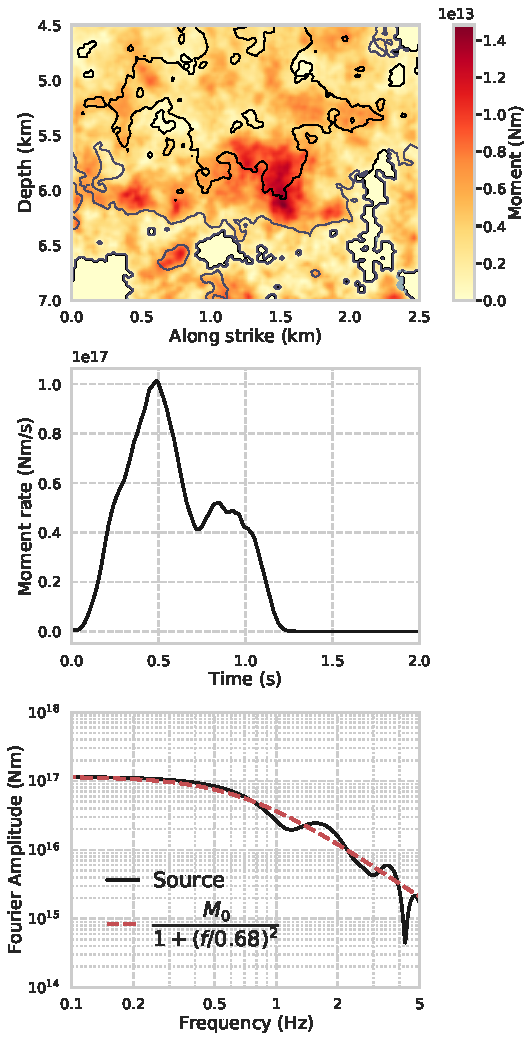
\includegraphics[width=0.9\textwidth,height=0.9\textheight,keepaspectratio]{figures/figure_vs30_2.pdf}
  \caption{Description of the selected source model used in this study. (a) Moment distribution (shading). The contours represent rupture time at a 0.4 s interval starting from 0. (b) and (c) represent the sum of the moment rates for all subfaults and the Fourier amplitude spectrum, respectively.  A Brune-type $\omega^{-2}$ decay source \citep{brune1970tectonic} that fits the source spectrum is plotted for reference.}
  \label{fig:vs30-2}
\end{figure}

\clearpage
\begin{figure}[!ht]
  \centering
  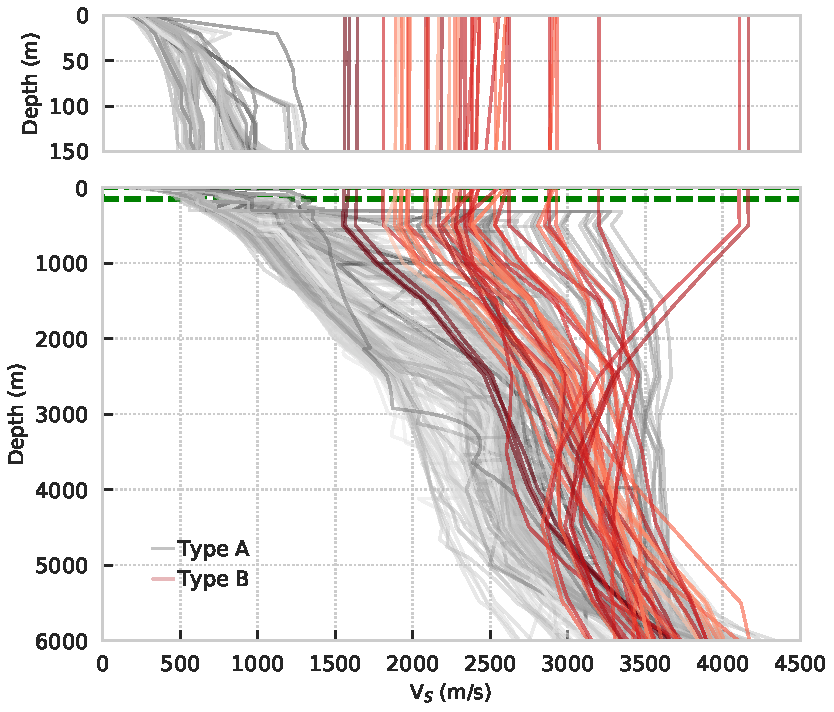
\includegraphics[width=0.9\textwidth]{figures/figure_vs30_3.pdf}
  \caption{(a) Top 150 m and (b) 0-4000 m $V_S$ profiles at the 259 stations. The black and red curves represent type B (surface $V_S >= 1000$ m/s) and soil (surface $V_S < 1000$ m/s) sites, respectively. The darker curves denote the sites with farther distance from the source.}
  \label{fig:vs30-3}
\end{figure}

\clearpage
\begin{figure}[!ht]
  \centering
  \includegraphics[width=0.9\textwidth]{figures/figure_vs30_4.pdf}
  \caption{FAS derived from the records (black) and CVM-S (blue) for the (a) east-west component, (b) north-south component and (c) vertical component. The left and right columns represent type A and B sites, respectively. The solid line is the median of FAS over the site group, the narrow band is the 95\% confidence interval of the median, and the dashed lines depict the standard deviation centered at the median.
  }
  \label{fig:vs30-4}
\end{figure}

\clearpage
\begin{figure}[!ht]
  \centering
  \includegraphics[width=0.9\textwidth]{figures/figure_vs30_5.png}
  \caption{(a) Surface $V_S$ extracted from CVM-S, and (b) $V_{S30}$ from \citet{thompsonUpdatedVs30Map2018} in our model domain (values in the left bottom corner are not available). The star denotes the epicenter.}
  \label{fig:vs30-5}
\end{figure}

\clearpage
\begin{figure}[!ht]
  \centering
  \includegraphics[width=0.9\textwidth]{figures/figure_vs30_6.pdf}
  \caption{Representative $V_S$ profiles for (a) type A sites and (b) type B sites from CVM-S. The thick black curves depict the averaged velocity profiles for all 220 type A and 39 type B sites directly extracted from CVM-S. The thin lines show the $V_S$ profiles resulting from our proposed method for different $z_T$ depths between 200 m and 1500 m. The dashed curve shows the $V_S$ profile calculated using the \Cref{eq:vs30-2} tapers from our preferred $z_T$ of 1000 m (note that because the tapers are applied as upper bounds to $V_S$, they typically only affect the type A $V_S$ structure at depths exceeding 350m, where the GTL in CVM-S ceases and causes the abrupt discontinuity).}
  \label{fig:vs30-6}
\end{figure}

\clearpage
\begin{figure}[!ht]
  \centering
  \includegraphics[width=0.9\textwidth]{figures/figure_vs30_7.pdf}
  \caption{The SH1D response for the refined profiles using various $z_T$ depths for average (a) type A and (b) type B sites, divided by the response obtained with the averaged type A and type B profiles from CVM-S.}
  \label{fig:vs30-7}
\end{figure}

\clearpage
\begin{figure}[!ht]
  \centering
  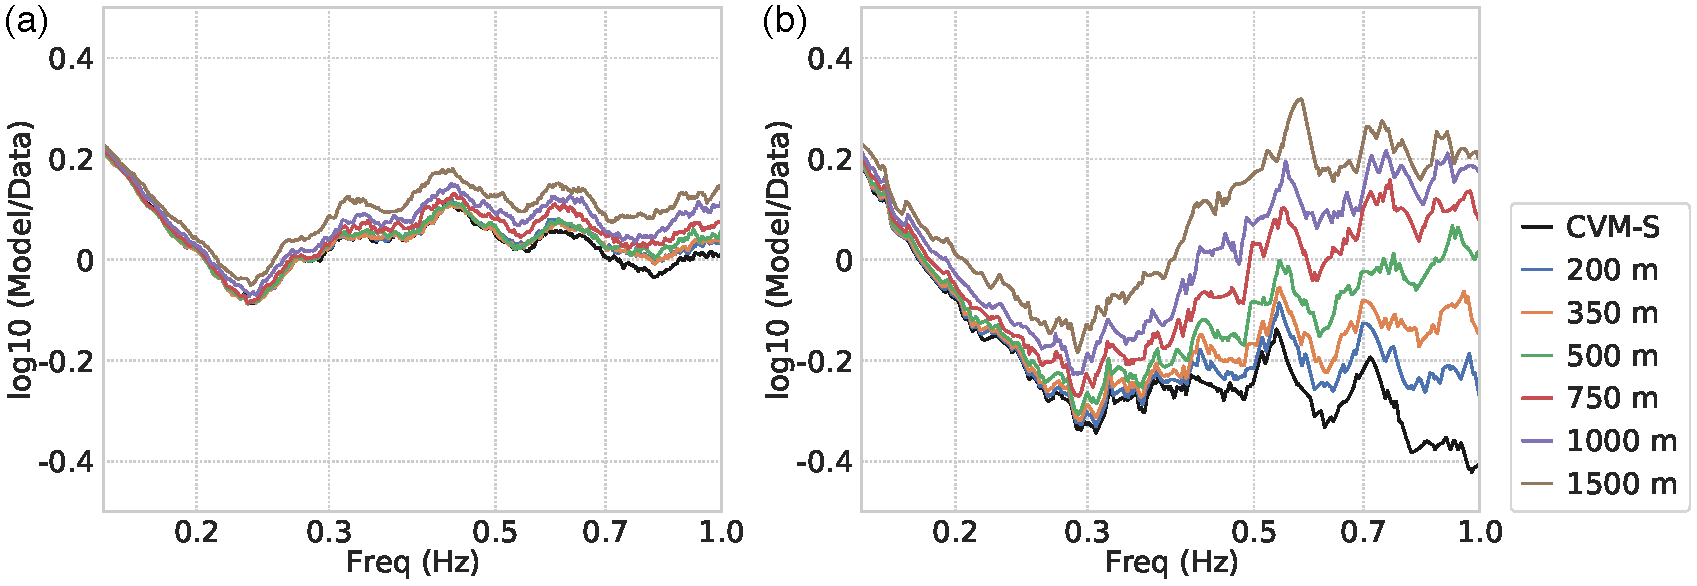
\includegraphics[width=0.9\textwidth]{figures/figure_vs30_8.pdf}
  \caption{Bias of FAS for the two horizontal components averaged over all (a) type A and (b) type B sites for CVM-S at all 259 stations, superimposed with the corresponding SH1D response. The black curves denote CVM-S and other labeled curves represent various tapering depths using SH1D results.}
  \label{fig:vs30-8}
\end{figure}

\clearpage
\begin{figure}[!ht]
  \centering
  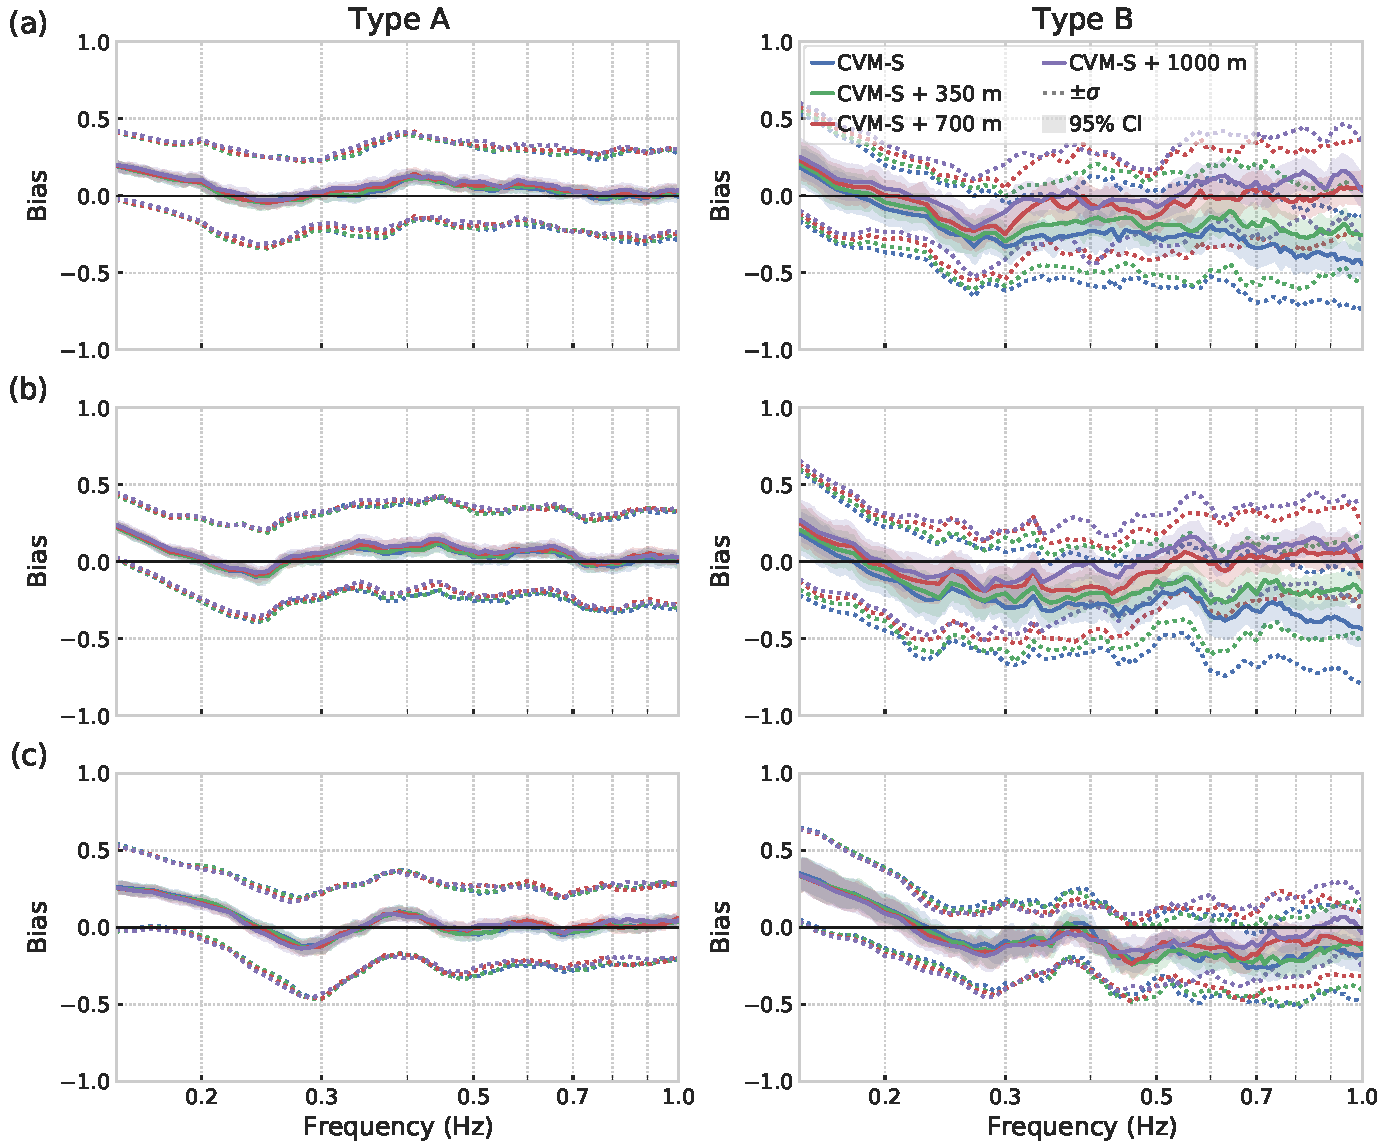
\includegraphics[width=0.9\textwidth]{figures/figure_vs30_9.pdf}
  \caption{Bias of FAS on the (a) east-west, (b) north-south and (c) vertical components, calculated from 3D simulations in CVM-S and with tapering depth of 350 m, 700 m, and 1000 m. A positive (negative) value depicts overprediction (underprediction). The left (right) column shows type A (B) sites. The solid line is the median of FAS, where the narrow band is the 95\% confidence interval of the median, and the dashed lines depict the standard deviation centered at the median.}
  \label{fig:vs30-9}
\end{figure}

\clearpage
\begin{figure}[!ht]
  \centering
  \includegraphics[width=0.9\textwidth]{figures/figure_vs30_10.png}
  \caption{Maps of interpolated log10-based FAS bias between four 3D models and data: (a) CVM-S, and CVM-S with tapering depth of (b) 350 m, (c) 700 m and (d) 1000 m, calculated from the synthetics and records at 259 stations. The warm (cool) colors represent overprediction (underprediction). The circles (triangles) depict type A (B) sites. Note the log10-based colorbar.}
  \label{fig:vs30-10}
\end{figure}

\clearpage
\begin{figure}[!ht]
  \centering
  \includegraphics[width=0.9\textwidth]{figures/figure_vs30_11.png}
  \caption{Maps of interpolated log10-based FAS bias for two 3D CVMs and data. (a) CVM-S with velocity tapering depth of 350 m and $Q_S=0.15V_S$, and (b) CVM-S with velocity tapering depth of 1000 m and $Q_S=0.05V_S$. Warm (cool) colors represent overprediction (underprediction). Circles depict type A sites and triangles show type B sites.}
  \label{fig:vs30-11}
\end{figure}

\clearpage
\begin{figure}[!ht]
  \centering
  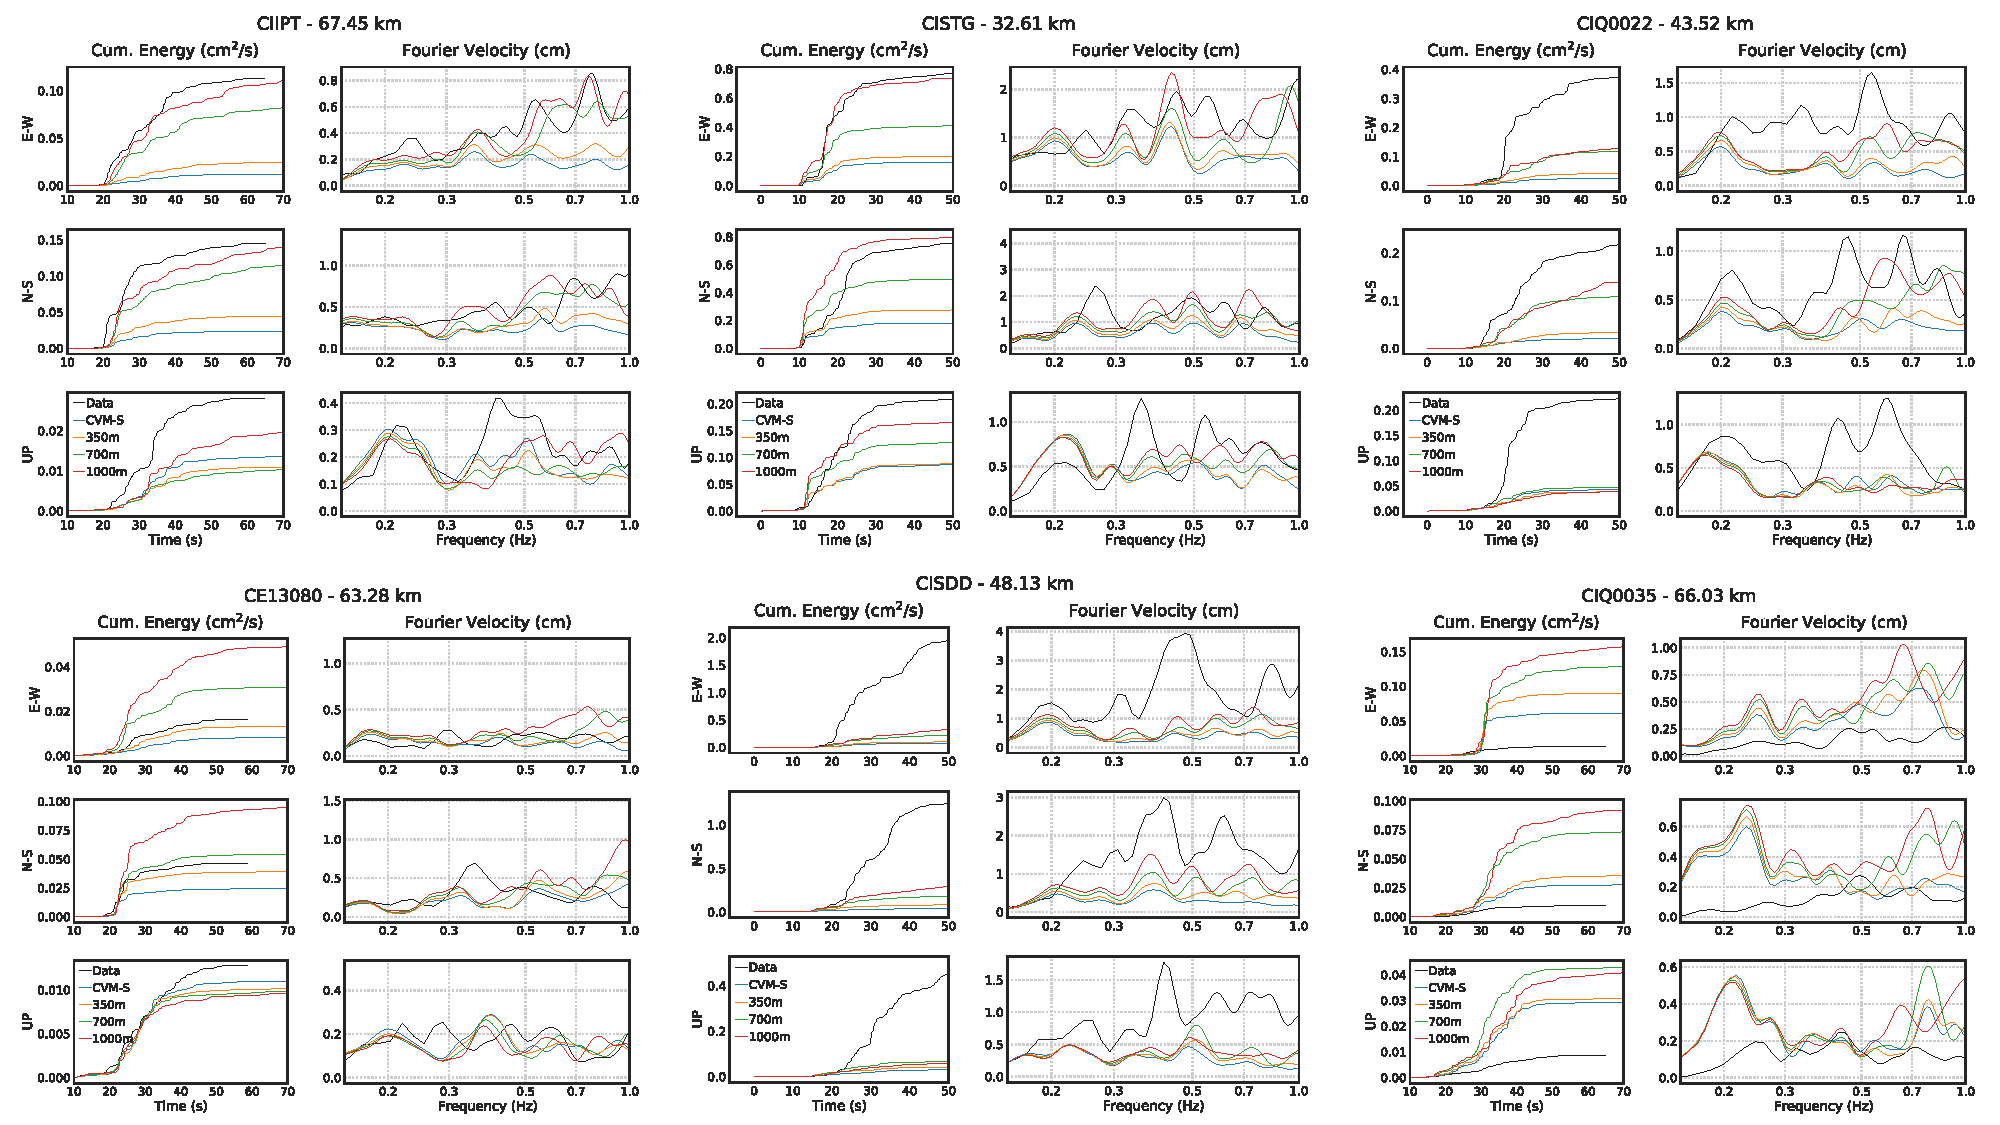
\includegraphics[width=0.9\textwidth]{figures/figure_vs30_12.pdf}
  \caption{Cumulative kinetic energy and Fourier velocity spectra at six type B sites. The subtitles show the names of the sites and their hypocentral distance.
  }
  \label{fig:vs30-12}
\end{figure}

\clearpage
\begin{figure}[!ht]
  \centering
  \includegraphics[width=0.9\textwidth]{figures/figure_vs30_13.pdf}
  \caption{Type B site $V_S$ profiles from CVM-S, and CVM-S and CVM-H with (default) \citet{elyVs30derivedNearsurfaceSeismic2010} GTL refinement depth of 350 m.}
  \label{fig:vs30-13}
\end{figure}

\clearpage
\floatsetup[figure]{style=plain,subcapbesideposition=top}
\begin{figure}[!ht]
  \sidesubfloat[]{\includegraphics[width=0.4\textwidth]{figures/figure_vs30_14a.png}\label{fig:vs30-14a}} \hfil
  \sidesubfloat[]{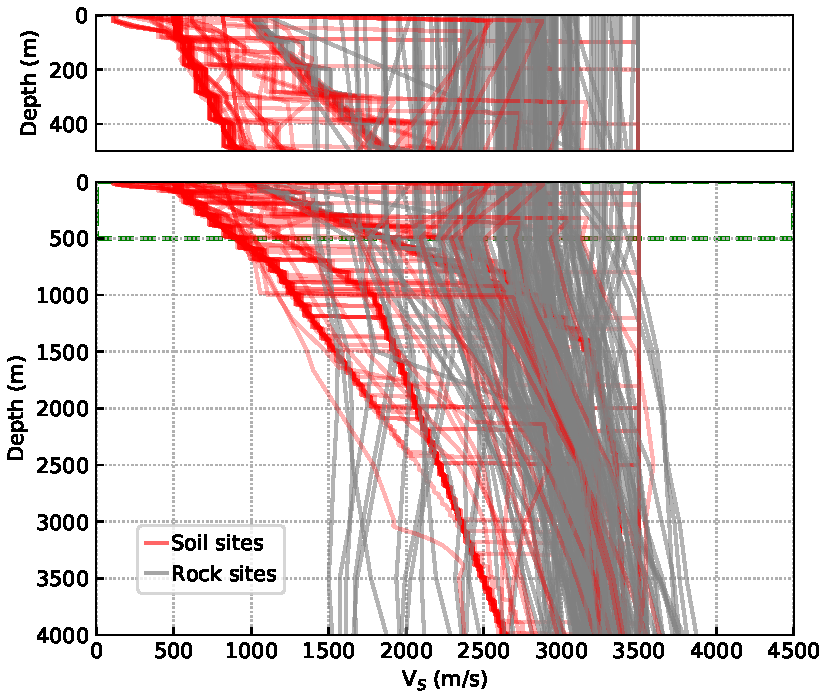
\includegraphics[width=0.45\textwidth]{figures/figure_vs30_14b.pdf}\label{fig:vs30-14b}} % \\[\baselineskip]%
  \caption{ (a) $V_S$ profile sample locations in California. Triangles denote type B sites and circles denote type A sites, and (b) extracted $V_S$ profiles. The top panel zooms into the top 500 m. }
  \label{fig:vs30-14}
\end{figure}


%% supplement
\setcounter{table}{0}
\setcounter{figure}{0}
\numberwithin{figure}{chapter}
\numberwithin{table}{chapter}
\renewcommand{\thetable}{A\arabic{chapter}.\arabic{table}}
\renewcommand{\thefigure}{A\arabic{chapter}.\arabic{figure}}
\newpage
\section*{Appendix}
\addcontentsline{toc}{section}{\protect\numberline{}Appendix}


%% Removed on 071821
% \begin{figure}[!ht]
%   \centering
%   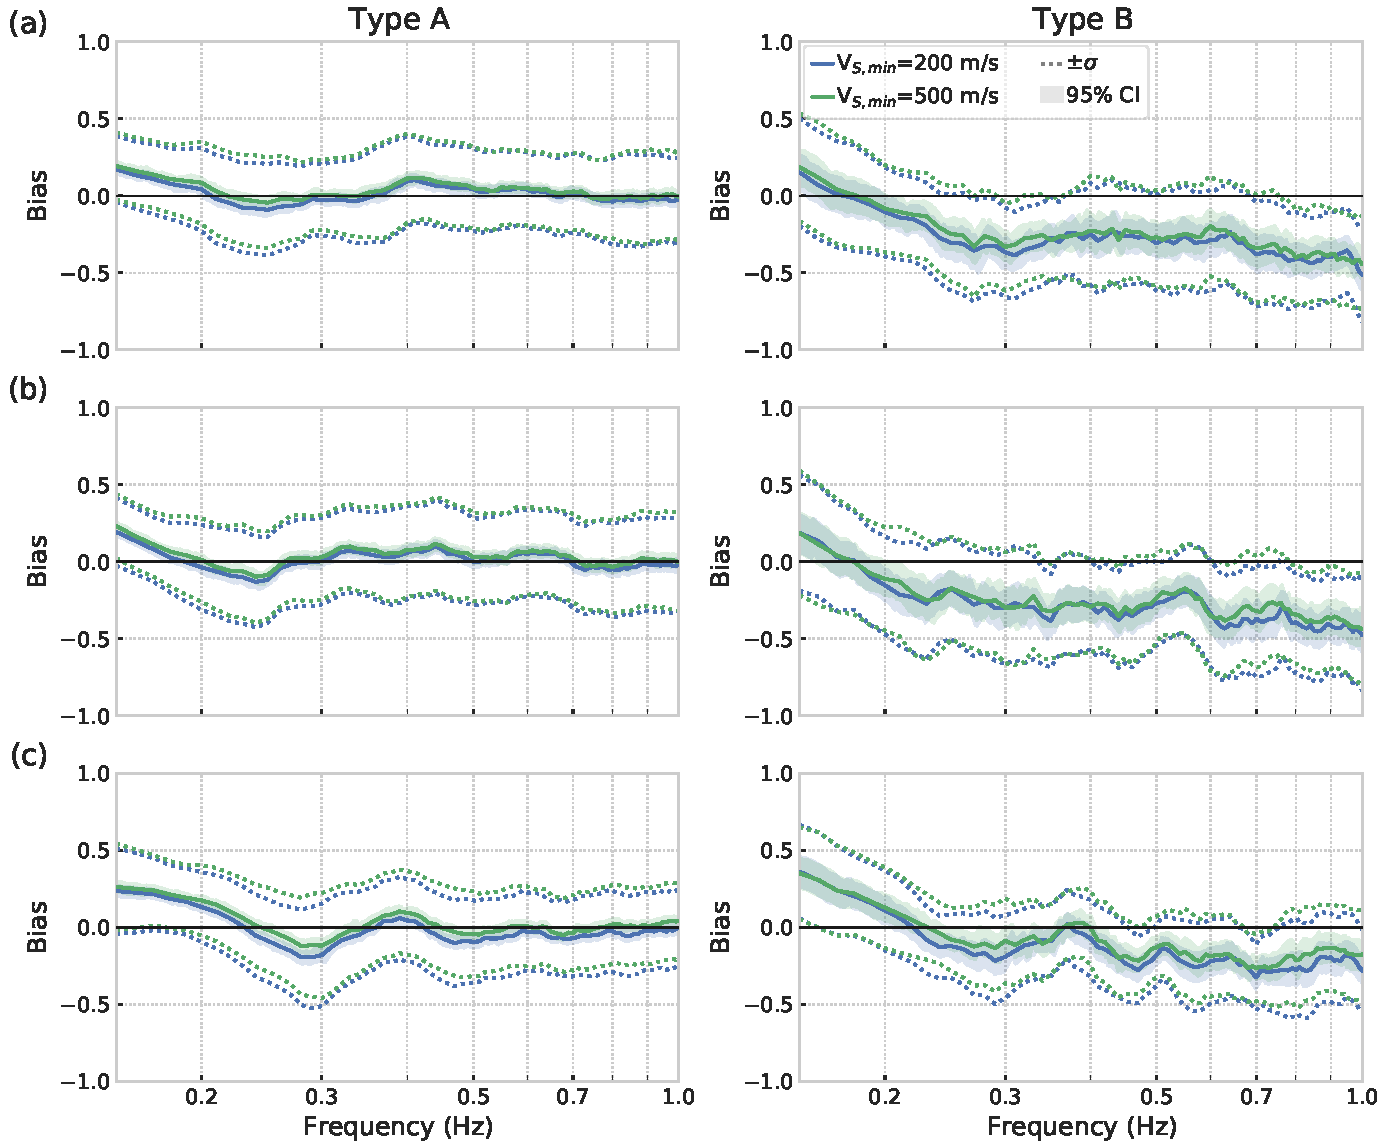
\includegraphics[width=0.9\textwidth]{figures/figure_vs30_S1.pdf}
%   \caption{Bias of FAS of the (a) east-west, (b) north-south and (c) vertical component, calculated from 3D simulations in CVM-S with minimum $V_S$ of 200 m/s (blue) and 500 m/s (green). A positive (negative) value means overprediction (underprediction). The left (right) columns show type A (B) sites. The solid line is the median of FAS, where the narrow band is the 95\% confidence interval of the median, and the dashed lines depict the standard deviation centered at the median.}
%   \label{fig:vs30-A1}
% \end{figure}
% \clearpage

\begin{figure}[!ht]
  \centering
  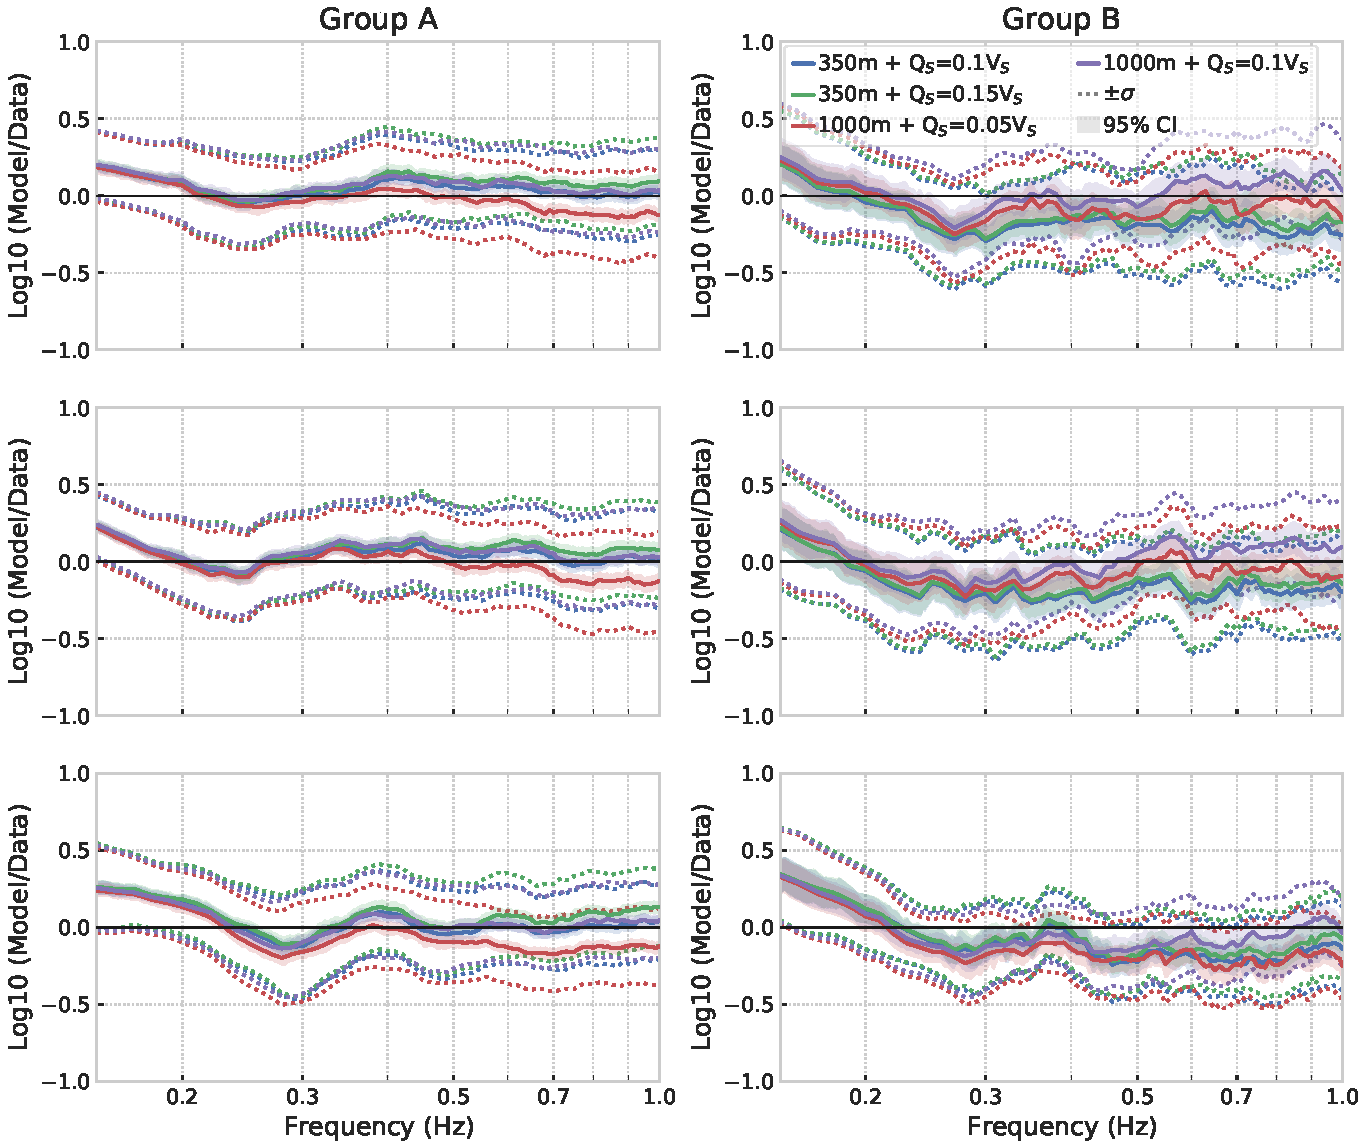
\includegraphics[width=0.9\textwidth]{figures/figure_vs30_S2.pdf}
  \caption{Bias of FAS of the (a) east-west, (b) north-south and (c) vertical component, calculated from 3D simulations in CVM-S with $V_S$ tapering depths of 350 m and 1000 m along with attenuation models $Q_S=0.05V_S$, $Q_S=0.1V_S$, and $Q_S=0.15V_S$. A positive (negative) value means overprediction (underprediction). The left (right) columns show type A (B) sites. The solid line is the median of FAS, where the narrow band is the 95\% confidence interval of the median, and the dashed lines depict the standard deviation centered at the median.}
  \label{fig:vs30-A2}
\end{figure}
\clearpage

\begin{figure}[!ht]
  \centering
  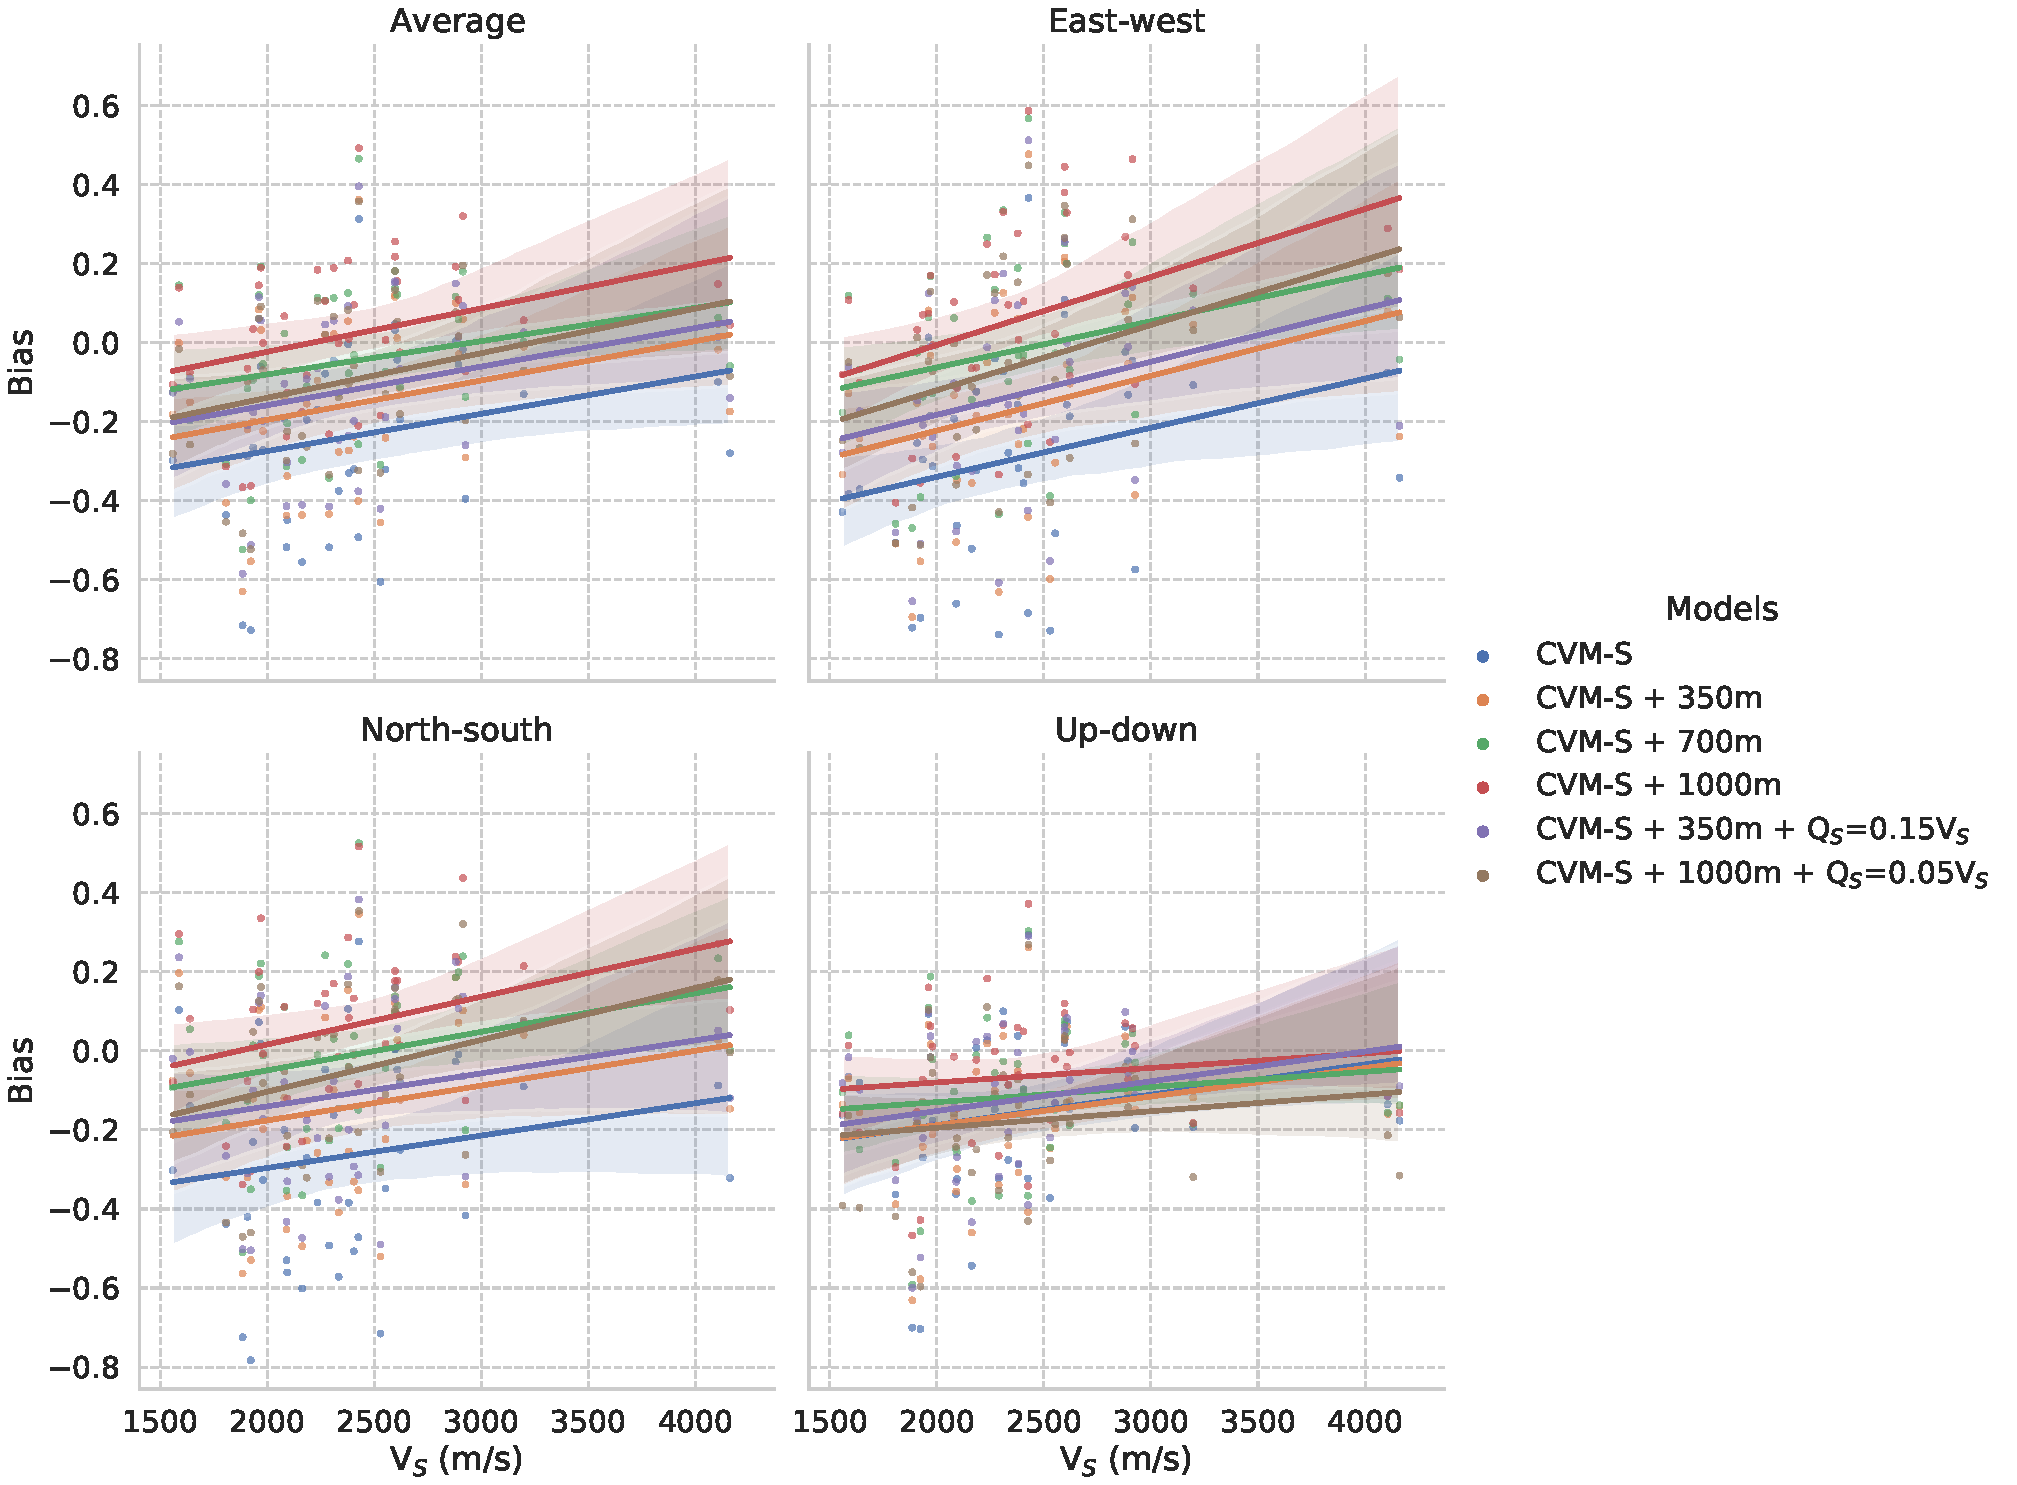
\includegraphics[width=0.9\textwidth]{figures/figure_vs30_S3.pdf}
  \caption{Averaged FAS bias for frequencies between 0.15-1 Hz at poorly constrained sites plotted as a function of site surface $V_S$ for (a) three-component average, (b) east-west, (c) north-south and (d) vertical components. The shades represent 95\% confidence intervals estimated using bootstrap.}
  \label{fig:vs30-A3}
\end{figure}


\renewcommand{\thetable}{\arabic{table}}
\renewcommand{\thefigure}{\arabic{figure}}

\numberwithin{figure}{chapter}
\numberwithin{table}{chapter}

%\endrefsection